\chapter{The Power Grid Control System}
%Control system
\section{The Conventional Power grid control system}
%- SCADA (historical)

%\subsection{The Classic SCADA subsystem}

The \acrshort{scada} system constituted the core part of the control center of the classic \acrlong{pg}, utilising one-directional communication lines in order to manually control and monitor the operational state of the power grid.

Figure \ref{fig:Blume-SCADA-system} shows the main components of the SCADA system.

\begin{figure}[ht]
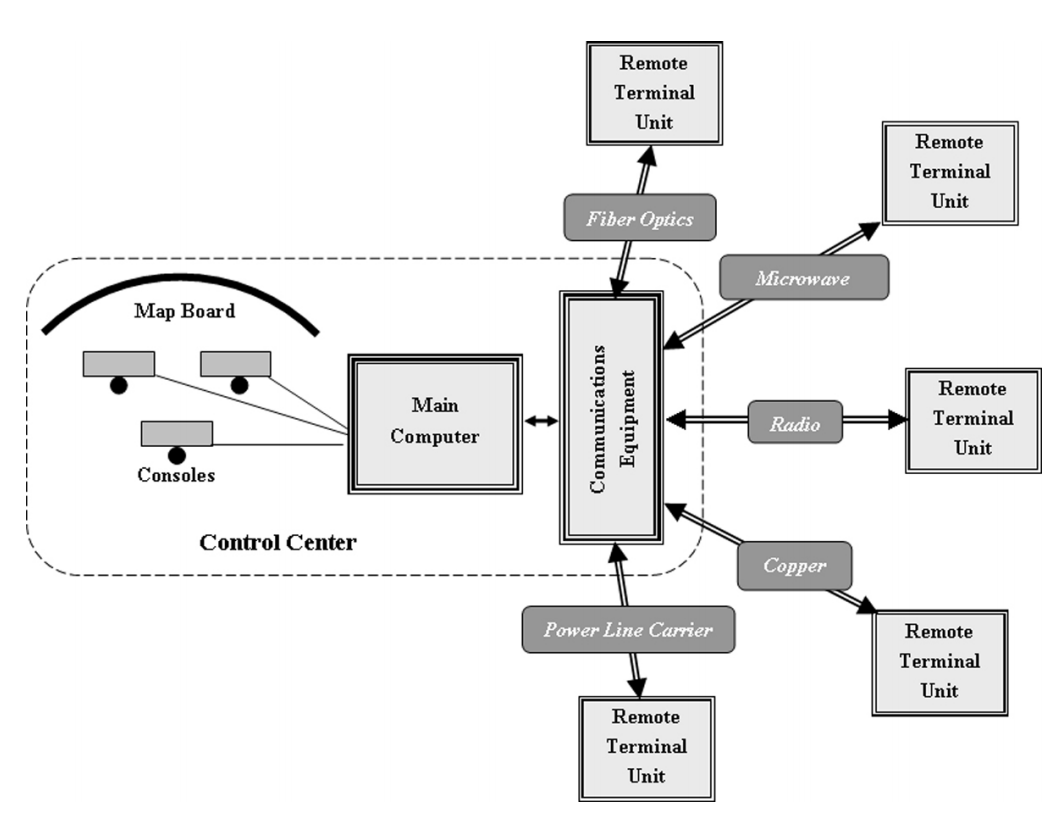
\includegraphics[width=\linewidth]{figures/Blume-SCADA-system.png}
\caption[SCADA system]{SCADA system , as presented in \cite{BlumeStevenW2007Epsb}}
\label{fig:Blume-SCADA-system}
\end{figure}

%[ \fullcite{el2008introduction} ] \\ 


A centrally located control center, optionally being backed up by control centers at one or more locations for redundancy, displays status information from the equipment at the associated substations, received for monitoring purposes. As a response to alarms indicating operational issues, commands enabling remote control of affected infrastructure is issued in order to address the issue, in order to resolve the issue and receive updated status information clearing the alarm. 




%\section{Description}
%- WAMS description

\section{The Smart Grid Control System}


\subsection{Introduction}

Analogous with the modernisation of the classic \acrlong{pg} into the \acrlong{sg}, the \acrshort{scada} subsystem of the \acrshort{pg} is the predecessor of the control system of the modern \acrlong{sg}.
Therefore, a description of the \acrshort{scada} system, evolving from the centralised subsystem controlling the Classic \acrshort{pg}, to the modernised version of the \acrshort{scada} subsystem, initiates the description of the \acrlong{sg} Control System. 




The characteristics of the three generations of SCADA systems% described by \Citeauthor{alcaraz2012security} in \cite{alcaraz2012security},
may be summarised below:
 

 \begin{enumerate}
     \item A Monolithic SCADA system utilises a centralised offline control center  infrastructure, in order to monitor and control the physical system by proprietary control mechanisms.
     \item A Distributed SCADA system utilises a networked, but centralised control  center in order to monitor and control the physical system by proprietary control mechanisms. 
     \item A Networked SCADA system utilises a networked, and online control  center in order to monitor and control the physical system by standardised control mechanisms.
 \end{enumerate}







\subsection{The Modernised SCADA system}
 
 The \acrshort{scada} system is%, as described in \cite{alcaraz2012security},
 a system utilised to supervise and control \acrfull{ci} systems, including \acrshort{pg} infrastructures. Initially designed in order to control physical infrastructure systems like the classic \acrlong{pg}, the Monolithic SCADA system emerged into the Distributed SCADA system. The transition from a Monolithic SCADA system to a Distributed SCADA system transforms, as indicated by %figure \ref{fig:SCADA-CentralisedAndDistributed}
 , the central management center from a centrally controlled mainframe environment, to a networked server environment controlled by operators connected through a \acrfull{lan}
  
  
 The \acrshort{sg} control center emerged from the Distributed SCADA system, into the Networked SCADA system used in order to control modern \acrlong{cps}s, like the \acrshort{sg}.\\ 
 


 





 




However, as explained by \Citeauthor{zamani2020introduction} in \Cite{zamani2020introduction}, the \acrshort{scada} system has a number of shortcomings, making it unsuitable for a \acrshort{sg} enegy distribution monitoring system:

\begin{itemize}
    \item The data polling rate is once every 2-10s, which is not sufficient in order to get real-time measurements.
    \item No time-stamps are attached to samples, making it hard to monitor rate of change over time
    \item State Estimation is not performed with sufficient frequency, if at all.
    \item The ability to observe dynamics is not supported by the system.
\end{itemize}





In order to address these shortcomings, the \acrfull{wams} system\footnote{WAMS is also known as the Wide Area \textbf{Monitoring} System}, described next, was invented.




\section{Wide Area Measurement System}
\begin{figure}[ht]
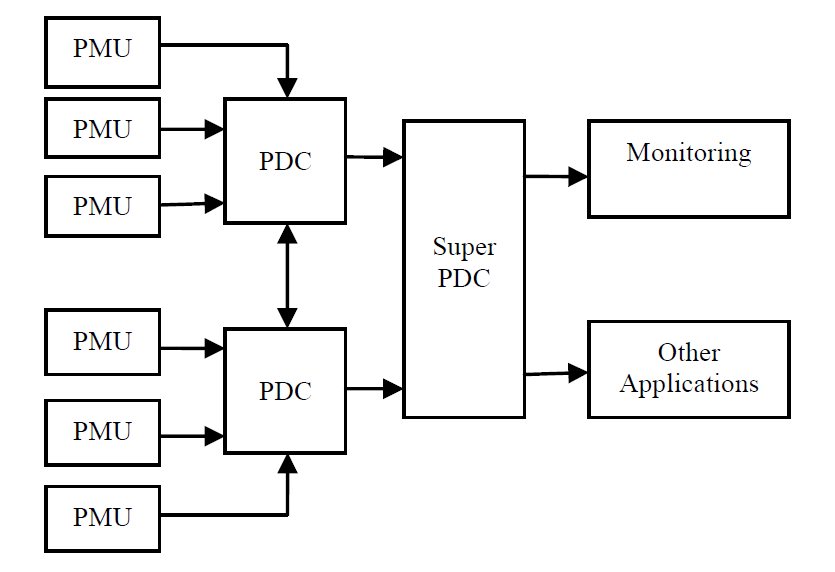
\includegraphics[width=\linewidth]{figures/Kumar-WAMS-architecture.png}
\caption[WAMS architecture]{WAMS architecture, as presented in \cite{kumar2015monitoring}}
\label{fig:Kumar-WAMS-architecture}
\end{figure}

   

In order to ensure the continuous monitoring of the modern \acrlong{sg} energy distribution system, the \acrfull{wams} is utilised. An overview of the \acrshort{wams} architecture, as presented in   \cite{kumar2015monitoring}, is shown as \figureautorefname  { } \ref{fig:Kumar-WAMS-architecture}:

The \acrshort{wams} is, as described in  \cite{kumar2015monitoring}, a  system, consisting of:

(1) \acrshort{pmu}s, (2) \acrshort{pdc}s, (3) The super \acrshort{pdc}, and (4) Communication networks.

The various components might be described as follows, from (4) to (1):
\begin{itemize}
    \item The \textbf{Communication Networks}, providing data transport between \acrshort{wams} components, as required.
    \item The \textbf{Super \acrshort{pdc}} controls several \acrshort{pdc}s constituting a distributed \acrshort{wams}.
\item The \textbf{\acrfull{pdc}} is responsible for collecting and interpreting \acrshort{pmu} measurements, before synchronising the measurements according to timestamps, in order to get more complete status information based on a combination of measurements.
    \item The \textbf{\acrfull{pmu}} is an intelligent measuring device, responsible for registering sensor measurements,  performing calculations like, for instance, phase angles, as well as voltage and current magnitudes. The data registered and processed by the \acrshort{pmu}, is transferred to the nearest \acrshort{pdc}.
    \end{itemize}





\section{Smart grid Monitoring}
The \acrlong{sg} system constitutes a complex system of subsystems, which proper operation is a prerequisite for the successful transmission of electric energy from producers to consumers. 
In order for the \acrshort{wams} to receive status monitoring data, a controlled process for retrieving and transmitting sensor data, is a prerequisite for proper system operation.



\subsection{Description of the Smart Grid  Monitoring system}
Electricity is produced according to the current demand for energy, as controlled by the Demand Management system, dynamically adjusting the energy supply accordingly. In order to successfully reply to the dynamically changing demands for energy, a close monitoring of the production, transmission and distribution of energy is required. In order for the monitoring system to obtain status information, the proper transmission of monitoring data from power status sensors to the   \acrshort{wams}  is essential.


%\section{Storing and transmitting data for monitoring}

\subsection{Phasor Measurment Units}
The \acrfull{pmu} is a system which receives samples from a number of sensors monitoring  real-time power line status, related to the electrical Voltage and Impedance the of the infrastructure being monitored. 
The entities monitored are known as electrical phases, most often part of a three-phase system, where each phase is separated by $120^0$.
Each \acrshort{pmu} is continuously calculating the phasor values of all sensors, alligning all values corresponding to a time stamp as synchrophasors, before transmitting a synchrophasor record for each timestamp to the single \acrfull{pdc} to which the \acrshort{pmu} has a  TCP or UDP network connection.

%target for the planned attack. 


%\subsection{Introduction}


\begin{figure}%[ht]
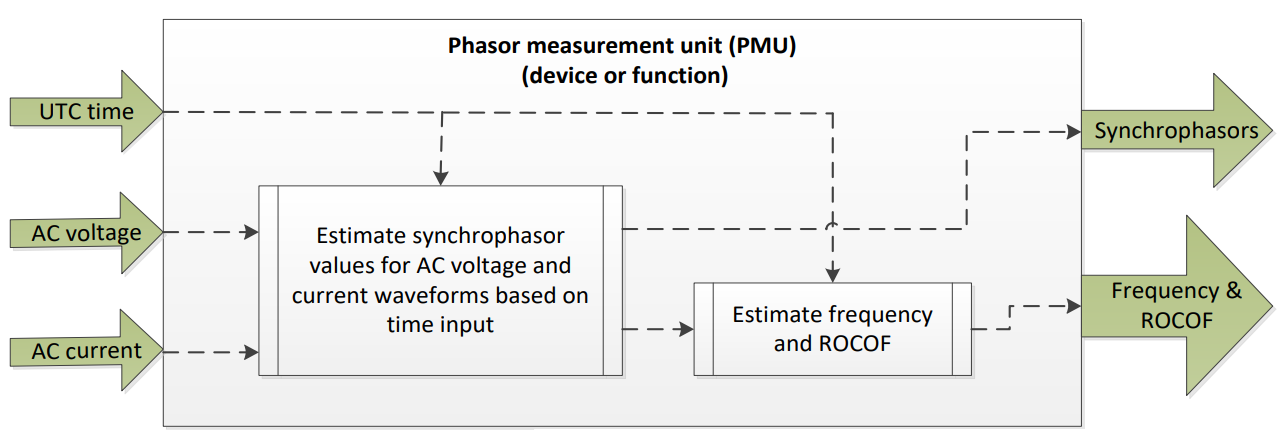
\includegraphics[width=\linewidth]{figures/PMU-in-out.png}
\caption[PMU inputs and outputs]{PMU inputs and outputs, as presented in \Cite[p.12]{iec2018measuring}
}
\label{fig:PMU-in-out}
\end{figure}

\subsection{Phasor data Concentrator}

The \acrfull{pdc} is a networked system responsible for forwarding synchronised phasor data from as number of \acrshort{pmu}s 
, to a more centralised \acrshort{pdc}, most often denoted a Super \acrshort{pdc}.



\
% In \cite{el2018cyber}, \citeauthor{el2018cyber} ...
 


%\subsection{Threats to security}
%In order to ensure the continuous operation of the \acrlong{sg}, identifying security vulnerabilities, and countering threats identified is of vital importance.  




\section{Advantages}
%  - advantages
\section{Security Issues}
%  - security issues
%\subsection{WAMS Security} 

The \acrfull{sg} \acrfull{wams} is a \acrshort{sg} subsystem enabling \acrshort{sg} system operators to monitor the state of \acrshort{sg} energy flow, and general system state. 
A vital requirement for the view of the current state of the \acrshort{sg} energy distribution to be correct is, as described in previous chapters, the ability of the \acrshort{wams} Super \acrshort{pdc}  to utilise synchrophasors collected from the \acrshort{pdc}s to produce a view of the system state. In order for the view to be correct, however, the correctness of the timestamps i critical.  Therefore, in order to produce correct time stamps, the reliability of the Time Synchronisation source is of Critical importance.


\section{State Estimation}

%  - State Estimation: Intro, to explain means to improve grid security.

%\section{WAMS state estimation}
In order to detect abnormalities or errors in the monitoring data received, the \acrshort{wams} includes applications capable of validating the quality of the state information received. Various state estimations exist, some of which give alerts on dubious system state based on comparisons with known good system states. State estimation systems increases the risk of attack detection, thus lowerses the probability of a threat actor being capable of pulling off a stealthy attack.   


